% answers.tex —— 2004 年·天津卷·文科 · 参考答案与详细解析片段
% 由 tools/generate_projects.py 依来源总账自 2004/2004_数学真题_天津文_试题.md + 2004/2004_数学真题_天津文_解析正文.md + 2004/2004_数学真题_天津文_答案要点.md 生成，勿手改（改源 MD 后重跑）


\begin{gktip}
固定源 PDF 为印刷页码 204–205 的两页题面，不附答案。以下解析均依据固定源独立推导复算；第 8、11、19 题图形在 LaTeX 工程中以 TikZ 矢量源重绘。
\end{gktip}

\begin{answer}
\gksolhead{1}{}

\textbf{题目}：

设集合 $P = \{1, 2, 3, 4, 5, 6\}$，$Q = \{x \in \mathbf{R} \mid 2 \le x \le 6\}$，那么下列结论正确的是\mbox{（　　）}

\begin{gkopts}(2)
\task A．$P \cap Q = P$
\task B．$P \cap Q \supseteq Q$
\task C．$P \cup Q = Q$
\task D．$P \cap Q \subsetneq P$
\end{gkopts}

\Needspace{4\baselineskip}
\textbf{解析}

已知集合 $P = \{1, 2, 3, 4, 5, 6\}$，$Q = \{x \in \mathbf{R} \mid 2 \le x \le 6\}$。
\Needspace{5\baselineskip}
求两集合的交集：
\nopagebreak[4]
\[
P \cap Q = \{2, 3, 4, 5, 6\}.
\]
逐项核对选项：
\begin{itemize}
\item 对于 A 选项：$1 \in P$ 但 $1 \notin Q$，故 $P \cap Q \neq P$，A 错误；
\item 对于 B 选项：集合 $Q$ 包含区间 $[2, 6]$ 内所有连续实数（如 $2.5 \in Q$），而 $P \cap Q$ 仅包含 5 个整数，故 $P \cap Q \not\supseteq Q$，B 错误；
\item 对于 C 选项：$1 \in P \subset P \cup Q$，但 $1 \notin Q$，故 $P \cup Q \neq Q$，C 错误；
\item 对于 D 选项：$P \cap Q = \{2, 3, 4, 5, 6\}$ 是集合 $P = \{1, 2, 3, 4, 5, 6\}$ 的真子集，即 $P \cap Q \subsetneq P$，D 正确。
\end{itemize}

故选 D。

\gkanswer{答案：D}

\end{answer}
\begin{answer}
\gksolhead{2}{}

\textbf{题目}：

不等式 $\dfrac{x-1}{x} \ge 2$ 的解集为\mbox{（　　）}

\begin{gkopts}(2)
\task A．$[-1, 0)$
\task B．$[-1, +\infty)$
\task C．$(-\infty, -1]$
\task D．$(-\infty, -1] \cup (0, +\infty)$
\end{gkopts}

\Needspace{4\baselineskip}
\textbf{解析}

\Needspace{5\baselineskip}
解分式不等式：
\nopagebreak[4]
\[
\dfrac{x-1}{x} \ge 2 \iff \dfrac{x-1}{x} - 2 \ge 0 \iff \dfrac{x-1-2x}{x} \ge 0 \iff \dfrac{-x-1}{x} \ge 0.
\]
\Needspace{5\baselineskip}
两边同乘以 $-1$，改变不等号方向：
\nopagebreak[4]
\[
\dfrac{x+1}{x} \le 0.
\]
\Needspace{5\baselineskip}
等价于整式不等式组：
\nopagebreak[4]
\[
\begin{cases}
(x+1)x \le 0, \\
x \neq 0,
\end{cases}
\iff -1 \le x < 0.
\]
因此解集为 $[-1, 0)$。

故选 A。

\gkanswer{答案：A}

\end{answer}
\begin{answer}
\gksolhead{3}{}

\textbf{题目}：

对任意实数 $a, b, c$，在下列命题中，真命题是\mbox{（　　）}

\begin{gkopts}(2)
\task A．“$ac > bc$”是“$a > b$”的必要条件
\task B．“$ac = bc$”是“$a = b$”的必要条件
\task C．“$ac > bc$”是“$a > b$”的充分条件
\task D．“$ac = bc$”是“$a = b$”的充分条件
\end{gkopts}

\Needspace{4\baselineskip}
\textbf{解析}

对任意实数 $a, b, c$，逐项分析各命题的真假：
\begin{itemize}
\item 对于 A 选项：“$ac > bc$”推不出“$a > b$”（例如当 $c < 0$ 时，$ac > bc \implies a < b$），反之“$a > b$”也推不出“$ac > bc$”（当 $c \le 0$ 时不成立），故“$ac > bc$”不是“$a > b$”的必要条件，A 错误；
\item 对于 B 选项：若 $a = b$，则由等式性质必有 $ac = bc$，即“$a = b \implies ac = bc$”，因此“$ac = bc$”是“$a = b$”的必要条件，B 正确；
\item 对于 C 选项：由 A 选项分析可知，若 $c = -1, a = 1, b = 2$，则 $ac = -1 > bc = -2$，但 $a < b$，充分性不成立，C 错误；
\item 对于 D 选项：若 $ac = bc$，当 $c = 0$ 时，$a, b$ 可取任意不相等的实数，推不出 $a = b$，充分性不成立，D 错误。
\end{itemize}

故选 B。

\gkanswer{答案：B}

\end{answer}
\begin{answer}
\gksolhead{4}{}

\textbf{题目}：

若平面向量 $\vec{b}$ 与向量 $\vec{a} = (1, -2)$ 的夹角是 $180^\circ$，且 $|\vec{b}| = 3\sqrt{5}$，则 $\vec{b} =$\mbox{（　　）}

\begin{gkopts}(4)
\task A．$(-3, 6)$
\task B．$(3, -6)$
\task C．$(6, -3)$
\task D．$(-6, 3)$
\end{gkopts}

\Needspace{4\baselineskip}
\textbf{解析}

已知平面向量 $\vec{a} = (1, -2)$。
\Needspace{5\baselineskip}
计算 $\vec{a}$ 的模长：
\nopagebreak[4]
\[
|\vec{a}| = \sqrt{1^2 + (-2)^2} = \sqrt{5}.
\]
\Needspace{5\baselineskip}
设向量 $\vec{b}$ 与 $\vec{a}$ 的夹角是 $180^\circ$，即 $\vec{b}$ 与 $\vec{a}$ 反向共线，可设：
\nopagebreak[4]
\[
\vec{b} = \lambda \vec{a} \quad (\lambda < 0).
\]
\Needspace{5\baselineskip}
由模长条件 $|\vec{b}| = 3\sqrt{5}$ 得：
\nopagebreak[4]
\[
|\vec{b}| = |\lambda||\vec{a}| = |\lambda|\sqrt{5} = 3\sqrt{5} \implies |\lambda| = 3.
\]
因为 $\lambda < 0$，所以 $\lambda = -3$。
\Needspace{5\baselineskip}
代入得：
\nopagebreak[4]
\[
\vec{b} = -3(1, -2) = (-3, 6).
\]

故选 A。

\gkanswer{答案：A}

\end{answer}
\begin{answer}
\gksolhead{5}{}

\textbf{题目}：

设 $P$ 是双曲线 $\dfrac{x^2}{a^2} - \dfrac{y^2}{9} = 1$ 上一点，双曲线的一条渐近线方程为 $3x - 2y = 0$，$F_1$、$F_2$ 分别是双曲线的左、右焦点，若 $|PF_1| = 3$，则 $|PF_2| =$\mbox{（　　）}

\begin{gkopts}(2)
\task A．$1$ 或 $5$
\task B．$6$
\task C．$7$
\task D．$9$
\end{gkopts}

\Needspace{4\baselineskip}
\textbf{解析}

双曲线方程为 $\dfrac{x^2}{a^2} - \dfrac{y^2}{9} = 1$。
\Needspace{5\baselineskip}
其焦点在 $x$ 轴上，渐近线方程为：
\nopagebreak[4]
\[
y = \pm \dfrac{3}{a}x.
\]
\Needspace{5\baselineskip}
已知一条渐近线方程为 $3x - 2y = 0 \iff y = \dfrac{3}{2}x$，对比得：
\nopagebreak[4]
\[
\dfrac{3}{a} = \dfrac{3}{2} \implies a = 2.
\]
因此实半轴长 $a = 2$，实轴长 $2a = 4$。
\Needspace{5\baselineskip}
根据双曲线的几何定义，双曲线上任意一点 $P$ 到两焦点 $F_1, F_2$ 的距离差的绝对值等于实轴长：
\nopagebreak[4]
\[
||PF_1| - |PF_2|| = 2a = 4.
\]
已知 $|PF_1| = 3$：
\begin{itemize}
\item 若点 $P$ 在双曲线右支上，则 $|PF_1| - |PF_2| = 4 \implies |PF_2| = |PF_1| - 4 = 3 - 4 = -1 < 0$，不合题意；
\item 若点 $P$ 在双曲线左支上，则 $|PF_2| - |PF_1| = 4 \implies |PF_2| = |PF_1| + 4 = 3 + 4 = 7$。
\end{itemize}

因此 $|PF_2| = 7$。

故选 C。

\gkanswer{答案：C}

\end{answer}
\begin{answer}
\gksolhead{6}{}

\textbf{题目}：

若函数 $f(x) = \log_a x$ ($0 < a < 1$) 在区间 $[a, 2a]$ 上的最大值是最小值的 3 倍，则 $a =$\mbox{（　　）}

\begin{gkopts}(2)
\task A．$\dfrac{\sqrt{2}}{4}$
\task B．$\dfrac{\sqrt{2}}{2}$
\task C．$\dfrac{1}{4}$
\task D．$\dfrac{1}{2}$
\end{gkopts}

\Needspace{4\baselineskip}
\textbf{解析}

函数 $f(x) = \log_a x$ ($0 < a < 1$)。
由于底数 $0 < a < 1$，$f(x)$ 在定义域上单调递减。
在区间 $[a, 2a]$ 上，$f(x)$ 严格递减，因此：
\begin{itemize}
\item 最大值为 $f(a) = \log_a a = 1$；
\item 最小值为 $f(2a) = \log_a(2a) = \log_a 2 + \log_a a = 1 + \log_a 2$。
\end{itemize}

\Needspace{5\baselineskip}
已知最大值是最小值的 3 倍：
\nopagebreak[4]
\[
1 = 3(1 + \log_a 2) \iff 1 + \log_a 2 = \dfrac{1}{3} \iff \log_a 2 = -\dfrac{2}{3}.
\]
\Needspace{5\baselineskip}
根据对数与指数互逆关系：
\nopagebreak[4]
\[
a^{-\frac{2}{3}} = 2 \iff a = 2^{-\frac{3}{2}} = \dfrac{1}{\sqrt{2^3}} = \dfrac{1}{2\sqrt{2}} = \dfrac{\sqrt{2}}{4}.
\]

故选 A。

\gkanswer{答案：A}

\end{answer}
\begin{answer}
\gksolhead{7}{}

\textbf{题目}：

若过定点 $M(-1, 0)$ 且斜率为 $k$ 的直线与圆 $x^2 + 4x + y^2 - 5 = 0$ 在第一象限内的部分有交点，则 $k$ 的取值范围是\mbox{（　　）}

\begin{gkopts}(2)
\task A．$0 < k < \sqrt{5}$
\task B．$-\sqrt{5} < k < 0$
\task C．$0 < k < \sqrt{13}$
\task D．$0 < k < 5$
\end{gkopts}

\Needspace{4\baselineskip}
\textbf{解析}

圆的方程为 $x^2 + 4x + y^2 - 5 = 0 \iff (x+2)^2 + y^2 = 9$。
圆心为 $C(-2, 0)$，半径 $R = 3$。
求圆与坐标轴的交点：
\begin{itemize}
\item 令 $y = 0$，得 $(x+2)^2 = 9 \implies x = 1$ 或 $x = -5$，圆与 $x$ 轴正半轴交于点 $A(1, 0)$；
\item 令 $x = 0$，得 $y^2 = 5 \implies y = \sqrt{5}$（第一象限），圆与 $y$ 轴正半轴交于点 $B(0, \sqrt{5})$。
\end{itemize}

圆在第一象限内的部分为开圆弧 $AB$（不含边界交点 $A(1, 0)$ 与 $B(0, \sqrt{5})$）。
过定点 $M(-1, 0)$ 且斜率为 $k$ 的直线方程为 $y = k(x+1)$：
\begin{itemize}
\item 当直线过点 $A(1, 0)$ 时：
\end{itemize}
\nopagebreak[4]
\[
k_{MA} = \dfrac{0 - 0}{1 - (-1)} = 0;
\]
\begin{itemize}
\item 当直线过点 $B(0, \sqrt{5})$ 时：
\end{itemize}
\nopagebreak[4]
\[
k_{MB} = \dfrac{\sqrt{5} - 0}{0 - (-1)} = \sqrt{5}.
\]

直线与第一象限内的圆弧段相交，结合图象可知直线斜率 $k$ 的取值范围为 $(0, \sqrt{5})$。

故选 A。

\gkanswer{答案：A}

\end{answer}
\begin{answer}
\gksolhead{8}{}

\textbf{题目}：

如图，定点 $A$ 和 $B$ 都在平面 $\alpha$ 内，定点 $P \notin \alpha$，$PB \perp \alpha$，$C$ 是 $\alpha$ 内异于 $A$ 和 $B$ 的动点，且 $PC \perp AC$．那么，动点 $C$ 在平面 $\alpha$ 内的轨迹是\mbox{（　　）}
\nopagebreak[4]
\begin{center}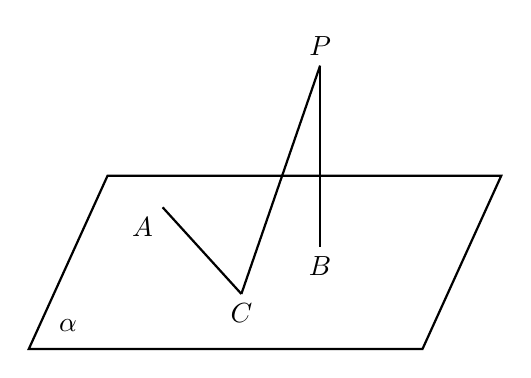
\begin{tikzpicture}[>=stealth, scale=1.0]
  % 平面 alpha
  \coordinate (M1) at (-0.5, -0.4);
  \coordinate (M2) at (4.5, -0.4);
  \coordinate (M3) at (5.5, 1.8);
  \coordinate (M4) at (0.5, 1.8);
  \draw[thick] (M1) -- (M2) -- (M3) -- (M4) -- cycle;
  \node at (0.0, -0.1) {$\alpha$};

  % 点坐标
  \coordinate (A) at (1.2, 1.4);
  \coordinate (B) at (3.2, 0.9);
  \coordinate (P) at (3.2, 3.2);
  \coordinate (C) at (2.2, 0.3);

  % 线段
  \draw[thick] (P) -- (B);
  \draw[thick] (P) -- (C);
  \draw[thick] (A) -- (C);

  % 节点标注
  \node[above] at (P) {$P$};
  \node[below] at (B) {$B$};
  \node[below left] at (A) {$A$};
  \node[below] at (C) {$C$};
\end{tikzpicture}
\end{center}
\nopagebreak[4]
\begin{gkopts}(2)
\task A．一条线段，但要去掉两个点
\task B．一个圆，但要去掉两个点
\task C．一个椭圆，但要去掉两个点
\task D．半圆，但要去掉两个点
\end{gkopts}

\Needspace{4\baselineskip}
\textbf{解析}
\nopagebreak[4]
\begin{center}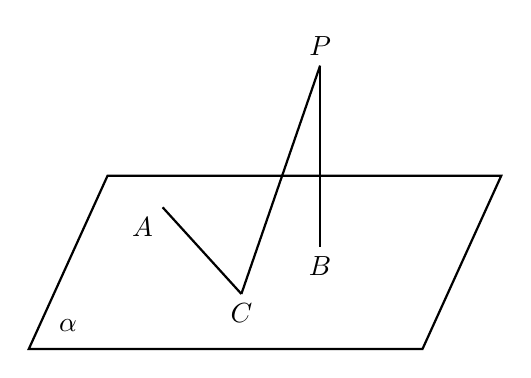
\begin{tikzpicture}[>=stealth, scale=1.0]
  % 平面 alpha
  \coordinate (M1) at (-0.5, -0.4);
  \coordinate (M2) at (4.5, -0.4);
  \coordinate (M3) at (5.5, 1.8);
  \coordinate (M4) at (0.5, 1.8);
  \draw[thick] (M1) -- (M2) -- (M3) -- (M4) -- cycle;
  \node at (0.0, -0.1) {$\alpha$};

  % 点坐标
  \coordinate (A) at (1.2, 1.4);
  \coordinate (B) at (3.2, 0.9);
  \coordinate (P) at (3.2, 3.2);
  \coordinate (C) at (2.2, 0.3);

  % 线段
  \draw[thick] (P) -- (B);
  \draw[thick] (P) -- (C);
  \draw[thick] (A) -- (C);

  % 节点标注
  \node[above] at (P) {$P$};
  \node[below] at (B) {$B$};
  \node[below left] at (A) {$A$};
  \node[below] at (C) {$C$};
\end{tikzpicture}
\end{center}
\nopagebreak[4]
由题设，$PB \perp \alpha$，而 $AC \subset \alpha$，所以 $PB \perp AC$。
又已知 $PC \perp AC$。
由于 $PB \cap PC = P$，$PB, PC \subset$ 平面 $PBC$，
\Needspace{5\baselineskip}
因此由线面垂直判定定理可知：
\nopagebreak[4]
\[
AC \perp \text{\text{平面} } PBC.
\]
\Needspace{5\baselineskip}
又 $BC \subset \text{\text{平面} } PBC$，所以：
\nopagebreak[4]
\[
AC \perp BC.
\]
在平面 $\alpha$ 内，点 $C$ 满足 $\angle ACB = 90^\circ$。
根据平面几何性质，对定线段 $AB$ 张直角的点 $C$ 的轨迹是以 $AB$ 为直径的圆。
因为题设指出 $C$ 是 $\alpha$ 内异于 $A$ 和 $B$ 的动点，故需去掉 $A, B$ 两个端点。
所以动点 $C$ 的轨迹是一个圆，但要去掉两个点。

故选 B。

\gkanswer{答案：B}

\end{answer}
\begin{answer}
\gksolhead{9}{}

\textbf{题目}：

函数 $y = 3^{x^2 - 1}$ ($-1 \le x < 0$) 的反函数是\mbox{（　　）}

\begin{gkopts}(1)
\task A．$y = \sqrt{1 + \log_3 x}$ ($x \ge \dfrac{1}{3}$)
\task B．$y = -\sqrt{1 + \log_3 x}$ ($x \ge \dfrac{1}{3}$)
\task C．$y = \sqrt{1 + \log_3 x}$ ($\dfrac{1}{3} < x \le 1$)
\task D．$y = -\sqrt{1 + \log_3 x}$ ($\dfrac{1}{3} < x \le 1$)
\end{gkopts}

\Needspace{4\baselineskip}
\textbf{解析}

已知原函数为 $y = 3^{x^2 - 1}$ ($-1 \le x < 0$)。
首先确定原函数的值域：
当 $-1 \le x < 0$ 时，$0 < x^2 \le 1$，
所以 $-1 < x^2 - 1 \le 0$。
因为底数 $3 > 1$，指数函数单调递增，
所以 $3^{-1} < 3^{x^2 - 1} \le 3^0 \iff \dfrac{1}{3} < y \le 1$。
即反函数的定义域为 $\left(\dfrac{1}{3}, 1\right]$。
\Needspace{5\baselineskip}
解关于 $x$ 的方程：
\nopagebreak[4]
\[
\log_3 y = x^2 - 1 \iff x^2 = 1 + \log_3 y.
\]
\Needspace{5\baselineskip}
因为 $x \in [-1, 0)$，所以取负根：
\nopagebreak[4]
\[
x = -\sqrt{1 + \log_3 y}.
\]
\Needspace{5\baselineskip}
互换自变量与因变量符号，得反函数方程为：
\nopagebreak[4]
\[
y = -\sqrt{1 + \log_3 x} \quad \left(\dfrac{1}{3} < x \le 1\right).
\]

故选 D。

\gkanswer{答案：D}

\end{answer}
\begin{answer}
\gksolhead{10}{}

\textbf{题目}：

函数 $y = 2\sin\left(\dfrac{\pi}{6} - 2x\right)$ ($x \in [0, \pi]$) 为增函数的区间是\mbox{（　　）}

\begin{gkopts}(1)
\task A．$\left[0, \dfrac{\pi}{3}\right]$
\task B．$\left[\dfrac{\pi}{12}, \dfrac{7\pi}{12}\right]$
\task C．$\left[\dfrac{\pi}{3}, \dfrac{5\pi}{6}\right]$
\task D．$\left[\dfrac{5\pi}{6}, \pi\right]$
\end{gkopts}

\Needspace{4\baselineskip}
\textbf{解析}

已知函数 $y = 2\sin\left(\dfrac{\pi}{6} - 2x\right) = -2\sin\left(2x - \dfrac{\pi}{6}\right)$ ($x \in [0, \pi]$)。
求该函数的单调递增区间，等价于求函数 $u = \sin\left(2x - \dfrac{\pi}{6}\right)$ 的单调递减区间。
\Needspace{5\baselineskip}
由正弦函数的递减区间性质：
\nopagebreak[4]
\[
2k\pi + \dfrac{\pi}{2} \le 2x - \dfrac{\pi}{6} \le 2k\pi + \dfrac{3\pi}{2} \quad (k \in \mathbf{Z}).
\]
\Needspace{5\baselineskip}
各项加上 $\dfrac{\pi}{6}$：
\nopagebreak[4]
\[
2k\pi + \dfrac{2\pi}{3} \le 2x \le 2k\pi + \dfrac{5\pi}{3}.
\]
\Needspace{5\baselineskip}
两边同除以 2：
\nopagebreak[4]
\[
k\pi + \dfrac{\pi}{3} \le x \le k\pi + \dfrac{5\pi}{6} \quad (k \in \mathbf{Z}).
\]
取 $k = 0$，得增区间为 $\left[\dfrac{\pi}{3}, \dfrac{5\pi}{6}\right]$。
该区间完全包含在给定定义域 $[0, \pi]$ 内。

故选 C。

\gkanswer{答案：C}

\end{answer}
\begin{answer}
\gksolhead{11}{}

\textbf{题目}：

如图，在长方体 $ABCD - A_1B_1C_1D_1$ 中，$AB = 6, AD = 4, AA_1 = 3$．分别过 $BC$、$A_1D_1$ 的两个平行截面将长方体分成三部分，其体积分别记为 $V_1 = V_{AEA_1-DFD_1}$，$V_2 = V_{EBE_1A_1-FCF_1D_1}$，$V_3 = V_{B_1E_1B-C_1F_1C}$．若 $V_1 : V_2 : V_3 = 1 : 4 : 1$，则截面 $A_1EFD_1$ 的面积为\mbox{（　　）}
\nopagebreak[4]
\begin{center}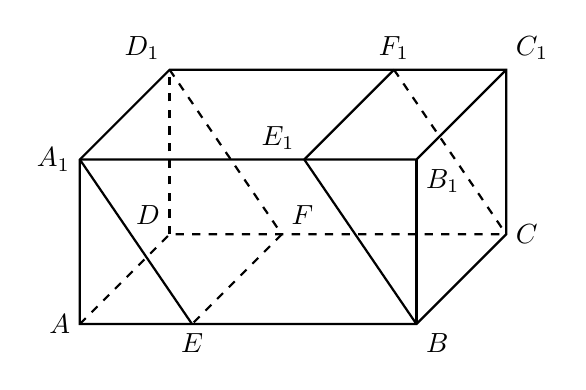
\begin{tikzpicture}[>=stealth, scale=0.95]
  % 顶点坐标
  \coordinate (A) at (0, 0);
  \coordinate (B) at (4.5, 0);
  \coordinate (C) at (5.7, 1.2);
  \coordinate (D) at (1.2, 1.2);

  \coordinate (A1) at (0, 2.2);
  \coordinate (B1) at (4.5, 2.2);
  \coordinate (C1) at (5.7, 3.4);
  \coordinate (D1) at (1.2, 3.4);

  % 截面分点 E, F, E1, F1 (比例 1:4:1, 即 1/6 与 5/6 处)
  % AB 长 4.5, E 在 1/3 (1.5) 处
  \coordinate (E) at (1.5, 0);
  \coordinate (F) at (2.7, 1.2);
  \coordinate (E1) at (3.0, 2.2);
  \coordinate (F1) at (4.2, 3.4);

  % 可见外框与实线
  \draw[thick] (A) -- (B) -- (C) -- (C1) -- (D1) -- (A1) -- cycle;
  \draw[thick] (A1) -- (B1) -- (C1);
  \draw[thick] (B) -- (B1);

  % 截面可见线
  \draw[thick] (A1) -- (E);
  \draw[thick] (E1) -- (B);
  \draw[thick] (E1) -- (F1);

  % 虚线（内部与被遮挡线）
  \draw[dashed, thick] (A) -- (D) -- (C);
  \draw[dashed, thick] (D) -- (D1);
  \draw[dashed, thick] (D1) -- (F) -- (E);
  \draw[dashed, thick] (F1) -- (C);

  % 节点标注
  \node[left] at (A) {$A$};
  \node[below right] at (B) {$B$};
  \node[right] at (C) {$C$};
  \node[above left] at (D) {$D$};

  \node[left] at (A1) {$A_1$};
  \node[below right] at (B1) {$B_1$};
  \node[above right] at (C1) {$C_1$};
  \node[above left] at (D1) {$D_1$};

  \node[below] at (E) {$E$};
  \node[above right] at (F) {$F$};
  \node[above left] at (E1) {$E_1$};
  \node[above] at (F1) {$F_1$};
\end{tikzpicture}
\end{center}
\nopagebreak[4]
\begin{gkopts}(4)
\task A．$4\sqrt{10}$
\task B．$8\sqrt{3}$
\task C．$4\sqrt{13}$
\task D．$16$
\end{gkopts}

\Needspace{4\baselineskip}
\textbf{解析}
\nopagebreak[4]
\begin{center}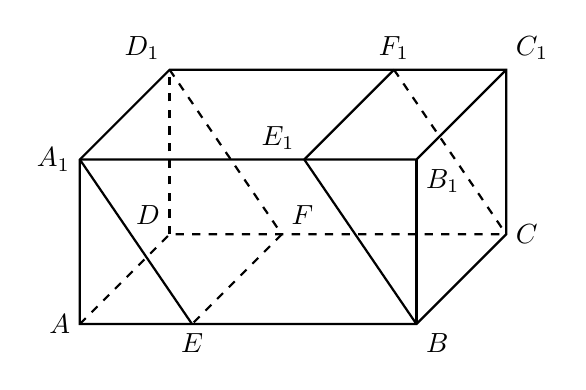
\begin{tikzpicture}[>=stealth, scale=0.95]
  % 顶点坐标
  \coordinate (A) at (0, 0);
  \coordinate (B) at (4.5, 0);
  \coordinate (C) at (5.7, 1.2);
  \coordinate (D) at (1.2, 1.2);

  \coordinate (A1) at (0, 2.2);
  \coordinate (B1) at (4.5, 2.2);
  \coordinate (C1) at (5.7, 3.4);
  \coordinate (D1) at (1.2, 3.4);

  % 截面分点 E, F, E1, F1 (比例 1:4:1, 即 1/6 与 5/6 处)
  % AB 长 4.5, E 在 1/3 (1.5) 处
  \coordinate (E) at (1.5, 0);
  \coordinate (F) at (2.7, 1.2);
  \coordinate (E1) at (3.0, 2.2);
  \coordinate (F1) at (4.2, 3.4);

  % 可见外框与实线
  \draw[thick] (A) -- (B) -- (C) -- (C1) -- (D1) -- (A1) -- cycle;
  \draw[thick] (A1) -- (B1) -- (C1);
  \draw[thick] (B) -- (B1);

  % 截面可见线
  \draw[thick] (A1) -- (E);
  \draw[thick] (E1) -- (B);
  \draw[thick] (E1) -- (F1);

  % 虚线（内部与被遮挡线）
  \draw[dashed, thick] (A) -- (D) -- (C);
  \draw[dashed, thick] (D) -- (D1);
  \draw[dashed, thick] (D1) -- (F) -- (E);
  \draw[dashed, thick] (F1) -- (C);

  % 节点标注
  \node[left] at (A) {$A$};
  \node[below right] at (B) {$B$};
  \node[right] at (C) {$C$};
  \node[above left] at (D) {$D$};

  \node[left] at (A1) {$A_1$};
  \node[below right] at (B1) {$B_1$};
  \node[above right] at (C1) {$C_1$};
  \node[above left] at (D1) {$D_1$};

  \node[below] at (E) {$E$};
  \node[above right] at (F) {$F$};
  \node[above left] at (E1) {$E_1$};
  \node[above] at (F1) {$F_1$};
\end{tikzpicture}
\end{center}
\nopagebreak[4]
在长方体 $ABCD - A_1B_1C_1D_1$ 中，棱长为 $AB = 6, AD = 4, AA_1 = 3$。
平行截面过 $A_1D_1$ 与 $BC$：
\begin{itemize}
\item 截面 $A_1EFD_1$ 过 $A_1D_1$，交底面于 $EF$，其中 $EF \parallel AD \parallel A_1D_1$；
\item 截面 $E_1BCF_1$ 过 $BC$，交顶面于 $E_1F_1$，其中 $E_1F_1 \parallel BC \parallel A_1D_1$。
\end{itemize}
因为两截面平行，在侧面 $ABB_1A_1$ 上有 $A_1E \parallel BE_1$。
长方体被分成三部分：
\begin{itemize}
\item $V_1 = V_{AEA_1-DFD_1}$ 为直三棱柱，高为 $AD = 4$，底面为直角三角形 $\triangle AEA_1$；
\item $V_3 = V_{B_1E_1B-C_1F_1C}$ 为直三棱柱，高为 $BC = 4$，底面为直角三角形 $\triangle B_1E_1B$；
\item $V_2 = V_{EBE_1A_1-FCF_1D_1}$ 为直四棱柱，高为 4，底面为平行四边形 $EBE_1A_1$。
\end{itemize}
\Needspace{5\baselineskip}
由于三部分在棱 $AD$ 方向的高均为 4，体积比等于侧面 $ABB_1A_1$ 上相应图形的面积比：
\nopagebreak[4]
\[
S_{\triangle AEA_1} : S_{EBE_1A_1} : S_{\triangle B_1E_1B} = V_1 : V_2 : V_3 = 1 : 4 : 1.
\]
矩形 $ABB_1A_1$ 的总面积为 $AB \cdot AA_1 = 6 \times 3 = 18$。
\Needspace{5\baselineskip}
总份数为 $1 + 4 + 1 = 6$，因此：
\nopagebreak[4]
\[
S_{\triangle AEA_1} = \dfrac{1}{6} \times 18 = 3.
\]
\Needspace{5\baselineskip}
在直角三角形 $\triangle AEA_1$ 中，$\angle A = 90^\circ$，$AA_1 = 3$：
\nopagebreak[4]
\[
S_{\triangle AEA_1} = \dfrac{1}{2} \cdot AE \cdot AA_1 = \dfrac{3}{2}AE = 3 \implies AE = 2.
\]
\Needspace{5\baselineskip}
由勾股定理，计算截面线段 $A_1E$ 的长：
\nopagebreak[4]
\[
A_1E = \sqrt{AE^2 + AA_1^2} = \sqrt{2^2 + 3^2} = \sqrt{13}.
\]
因为截面 $A_1EFD_1$ 是矩形，其边长分别为 $A_1D_1 = AD = 4$ 和 $A_1E = \sqrt{13}$，
\Needspace{5\baselineskip}
所以截面面积为：
\nopagebreak[4]
\[
S = A_1D_1 \cdot A_1E = 4\sqrt{13}.
\]

故选 C。

\gkanswer{答案：C}

\end{answer}
\begin{answer}
\gksolhead{12}{}

\textbf{题目}：

定义在 $\mathbf{R}$ 上的函数 $f(x)$ 既是偶函数又是周期函数，若 $f(x)$ 的最小正周期是 $\pi$，且当 $x \in \left[0, \dfrac{\pi}{2}\right]$ 时，$f(x) = \sin x$，则 $f\left(\dfrac{5\pi}{3}\right)$ 的值为\mbox{（　　）}

\begin{gkopts}(2)
\task A．$-\dfrac{1}{2}$
\task B．$\dfrac{1}{2}$
\task C．$-\dfrac{\sqrt{3}}{2}$
\task D．$\dfrac{\sqrt{3}}{2}$
\end{gkopts}

\Needspace{4\baselineskip}
\textbf{解析}

已知函数 $f(x)$ 既是偶函数又是周期函数，其最小正周期为 $\pi$。
\Needspace{5\baselineskip}
利用周期性化简：
\nopagebreak[4]
\[
f\left(\dfrac{5\pi}{3}\right) = f\left(\dfrac{5\pi}{3} - 2\pi\right) = f\left(-\dfrac{\pi}{3}\right).
\]
\Needspace{5\baselineskip}
由 $f(x)$ 是偶函数，得 $f(-x) = f(x)$，故：
\nopagebreak[4]
\[
f\left(-\dfrac{\pi}{3}\right) = f\left(\dfrac{\pi}{3}\right).
\]
\Needspace{5\baselineskip}
因为 $\dfrac{\pi}{3} \in \left[0, \dfrac{\pi}{2}\right]$，根据已知解析式 $f(x) = \sin x$：
\nopagebreak[4]
\[
f\left(\dfrac{\pi}{3}\right) = \sin\dfrac{\pi}{3} = \dfrac{\sqrt{3}}{2}.
\]

故选 D。

\gkanswer{答案：D}

\end{answer}
\begin{answer}
\gksolhead{13}{}

\textbf{题目}：

某工厂生产 A、B、C 三种不同型号的产品，产品数量之比依次为 $2 : 3 : 5$，现用分层抽样方法抽出一个容量为 $n$ 的样本，样本中 A 种型号产品有 16 件．那么此样本的容量 $n = \underline{\hspace{3em}}$．

\Needspace{4\baselineskip}
\textbf{解析}

三种型号产品数量比为 $2 : 3 : 5$，总份数为 $2 + 3 + 5 = 10$。
\Needspace{5\baselineskip}
在分层抽样中，各层所抽取的比例相等，A 种型号产品在总体中所占比例为：
\nopagebreak[4]
\[
\dfrac{2}{2 + 3 + 5} = \dfrac{2}{10} = \dfrac{1}{5}.
\]
\Needspace{5\baselineskip}
设样本容量为 $n$，则 A 种型号抽取件数为：
\nopagebreak[4]
\[
n \times \dfrac{1}{5} = 16 \implies n = 80.
\]

故答案为：80。

\gkanswer{答案：80}

\end{answer}
\begin{answer}
\gksolhead{14}{}

\textbf{题目}：

已知向量 $\vec{a} = (1, 1), \vec{b} = (2, -3)$，若 $k\vec{a} - 2\vec{b}$ 与 $\vec{a}$ 垂直，则实数 $k$ 等于 $\underline{\hspace{3em}}$．

\Needspace{4\baselineskip}
\textbf{解析}

已知向量 $\vec{a} = (1, 1), \vec{b} = (2, -3)$。
\Needspace{5\baselineskip}
计算线性组合向量：
\nopagebreak[4]
\[
k\vec{a} - 2\vec{b} = k(1, 1) - 2(2, -3) = (k - 4, k + 6).
\]
\Needspace{5\baselineskip}
因为 $k\vec{a} - 2\vec{b}$ 与 $\vec{a}$ 垂直，所以数量积为 0：
\nopagebreak[4]
\[
(k\vec{a} - 2\vec{b}) \cdot \vec{a} = 1 \cdot (k - 4) + 1 \cdot (k + 6) = 2k + 2 = 0 \implies k = -1.
\]

故答案为：-1。

\gkanswer{答案：-1}

\end{answer}
\begin{answer}
\gksolhead{15}{}

\textbf{题目}：

如果过两点 $A(a, 0)$ 和 $B(0, a)$ 的直线与抛物线 $y = x^2 - 2x - 3$ 没有交点，那么实数 $a$ 的取值范围是 $\underline{\hspace{3em}}$．

\Needspace{4\baselineskip}
\textbf{解析}

过两点 $A(a, 0)$ 和 $B(0, a)$ 的直线：
由题设知 $a \neq 0$（若 $a = 0$ 则两点重合不能确定直线）。
\Needspace{5\baselineskip}
直线的截距式方程为：
\nopagebreak[4]
\[
\dfrac{x}{a} + \dfrac{y}{a} = 1 \iff x + y = a \iff y = -x + a.
\]
\Needspace{5\baselineskip}
直线与抛物线 $y = x^2 - 2x - 3$ 没有交点，联立方程：
\nopagebreak[4]
\[
x^2 - 2x - 3 = -x + a \iff x^2 - x - (a + 3) = 0.
\]
\Needspace{5\baselineskip}
该二次方程无实根，等价于判别式严格小于 0：
\nopagebreak[4]
\[
\Delta = (-1)^2 - 4 \times 1 \times [-(a + 3)] = 1 + 4(a + 3) = 4a + 13 < 0 \iff a < -\dfrac{13}{4}.
\]
此时必有 $a < 0$，自然满足 $a \neq 0$。

故答案为：$\left(-\infty, -\dfrac{13}{4}\right)$。

\gkanswer{答案：$\left(-\infty, -\dfrac{13}{4}\right)$}

\end{answer}
\begin{answer}
\gksolhead{16}{}

\textbf{题目}：

从 0, 1, 2, 3, 4, 5 中任取 3 个数字，组成没有重复数字的三位数，其中能被 5 整除的三位数共有 $\underline{\hspace{3em}}$ 个．（用数字作答）

\Needspace{4\baselineskip}
\textbf{解析}

从集合 $\{0, 1, 2, 3, 4, 5\}$ 中任取 3 个不同数字组成三位数。
能被 5 整除的整数其个位数字必须是 0 或 5，分两类讨论：
1. 个位数字为 0：
\begin{itemize}
\item 百位数字可从 $\{1, 2, 3, 4, 5\}$ 中任选 1 个，有 5 种选法；
\item 十位数字从剩下的 4 个非零数字中任选 1 个，有 4 种选法；
\item 此类三位数共有 $5 \times 4 = 20$ 个。
\end{itemize}
2. 个位数字为 5：
\begin{itemize}
\item 百位数字不能为 0，只能从 $\{1, 2, 3, 4\}$ 中任选 1 个，有 4 种选法；
\item 十位数字可从 0 以及剩下的 3 个非零数字中任选 1 个，共有 4 种选法；
\item 此类三位数共有 $4 \times 4 = 16$ 个。
\end{itemize}

\Needspace{5\baselineskip}
两类互斥相加，符合条件的三位数共有：
\nopagebreak[4]
\[
20 + 16 = 36 \text{ \text{个}}.
\]

故答案为：36。

\gkanswer{答案：36}

\end{answer}
\begin{answer}
\gksolhead{17}{}

\textbf{题目}（本小题满分 12 分）：

已知 $\tan\left(\dfrac{\pi}{4} + \alpha\right) = \dfrac{1}{2}$．
（1）求 $\tan\alpha$ 的值；
（2）求 $\dfrac{\sin 2\alpha - \cos^2\alpha}{1 + \cos 2\alpha}$ 的值．

\Needspace{4\baselineskip}
\textbf{解析}

\Needspace{5\baselineskip}
（1）由两角和的正切公式：
\nopagebreak[4]
\[
\tan\left(\dfrac{\pi}{4} + \alpha\right) = \dfrac{\tan\dfrac{\pi}{4} + \tan\alpha}{1 - \tan\dfrac{\pi}{4}\tan\alpha} = \dfrac{1 + \tan\alpha}{1 - \tan\alpha}.
\]
\Needspace{5\baselineskip}
已知 $\tan\left(\dfrac{\pi}{4} + \alpha\right) = \dfrac{1}{2}$，得：
\nopagebreak[4]
\[
\dfrac{1 + \tan\alpha}{1 - \tan\alpha} = \dfrac{1}{2} \iff 2(1 + \tan\alpha) = 1 - \tan\alpha \iff 3\tan\alpha = -1 \iff \tan\alpha = -\dfrac{1}{3}.
\]

（2）利用二倍角公式化简目标式：
\Needspace{5\baselineskip}
分母为：
\nopagebreak[4]
\[
1 + \cos 2\alpha = 1 + (2\cos^2\alpha - 1) = 2\cos^2\alpha.
\]
\Needspace{5\baselineskip}
分子为：
\nopagebreak[4]
\[
\sin 2\alpha - \cos^2\alpha = 2\sin\alpha\cos\alpha - \cos^2\alpha.
\]
\Needspace{5\baselineskip}
代入分式中：
\nopagebreak[4]
\[
\dfrac{\sin 2\alpha - \cos^2\alpha}{1 + \cos 2\alpha} = \dfrac{2\sin\alpha\cos\alpha - \cos^2\alpha}{2\cos^2\alpha} = \dfrac{\sin\alpha}{\cos\alpha} - \dfrac{1}{2} = \tan\alpha - \dfrac{1}{2}.
\]
\Needspace{5\baselineskip}
将 $\tan\alpha = -\dfrac{1}{3}$ 代入，得：
\nopagebreak[4]
\[
\tan\alpha - \dfrac{1}{2} = -\dfrac{1}{3} - \dfrac{1}{2} = -\dfrac{5}{6}.
\]

\gkanswer{答案：（1）$-\dfrac{1}{3}$；（2）$-\dfrac{5}{6}$}

\end{answer}
\begin{answer}
\gksolhead{18}{}

\textbf{题目}（本小题满分 12 分）：

从 4 名男生和 2 名女生中任选 3 人参加演讲比赛．
（1）求所选 3 人都是男生的概率；
（2）求所选 3 人中恰有 1 名女生的概率；
（3）求所选 3 人中至少有 1 名女生的概率．

\Needspace{4\baselineskip}
\textbf{解析}

\Needspace{5\baselineskip}
从 4 名男生和 2 名女生共 6 人中任选 3 人参加比赛，基本事件总数为：
\nopagebreak[4]
\[
n = C_6^3 = \dfrac{6 \times 5 \times 4}{3 \times 2 \times 1} = 20.
\]

\Needspace{5\baselineskip}
（1）所选 3 人都是男生的基本事件数为：
\nopagebreak[4]
\[
m_1 = C_4^3 = 4.
\]
\Needspace{5\baselineskip}
所以所选 3 人都是男生的概率为：
\nopagebreak[4]
\[
P_1 = \dfrac{m_1}{n} = \dfrac{4}{20} = \dfrac{1}{5}.
\]

\Needspace{5\baselineskip}
（2）所选 3 人中恰有 1 名女生的事件相当于“1 女 2 男”，其基本事件数为：
\nopagebreak[4]
\[
m_2 = C_2^1 C_4^2 = 2 \times \dfrac{4 \times 3}{2 \times 1} = 2 \times 6 = 12.
\]
\Needspace{5\baselineskip}
所以所选 3 人中恰有 1 名女生的概率为：
\nopagebreak[4]
\[
P_2 = \dfrac{m_2}{n} = \dfrac{12}{20} = \dfrac{3}{5}.
\]

（3）“所选 3 人中至少有 1 名女生”的对立事件是“所选 3 人全是男生”。
\Needspace{5\baselineskip}
根据对立事件概率公式：
\nopagebreak[4]
\[
P_3 = 1 - P_1 = 1 - \dfrac{1}{5} = \dfrac{4}{5}.
\]

\gkanswer{答案：（1）$\dfrac{1}{5}$；（2）$\dfrac{3}{5}$；（3）$\dfrac{4}{5}$}

\end{answer}
\begin{answer}
\gksolhead{19}{}

\textbf{题目}（本小题满分 12 分）：

如图，在四棱锥 $P - ABCD$ 中，底面 $ABCD$ 是正方形，侧棱 $PD \perp \text{\text{底面} } ABCD$，$PD = DC$，$E$ 是 $PC$ 的中点．
（1）证明：$PA \parallel \text{\text{平面} } EDB$；
（2）求 $EB$ 与底面 $ABCD$ 所成角的正切值．
\nopagebreak[4]
\begin{center}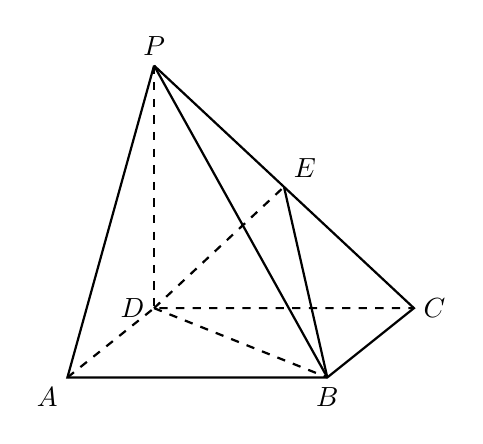
\begin{tikzpicture}[>=stealth, scale=1.1]
  % 顶点坐标
  \coordinate (D) at (1.0, 0.8);
  \coordinate (A) at (0, 0);
  \coordinate (B) at (3.0, 0);
  \coordinate (C) at (4.0, 0.8);
  \coordinate (P) at (1.0, 3.6);

  % 中点 E (PC 中点): P(1.0, 3.6), C(4.0, 0.8) -> E(2.5, 2.2)
  \coordinate (E) at (2.5, 2.2);

  % 实线棱
  \draw[thick] (P) -- (A) -- (B) -- (C) -- (P);
  \draw[thick] (P) -- (B);
  \draw[thick] (E) -- (B);

  % 虚线棱与辅助线
  \draw[dashed, thick] (P) -- (D);
  \draw[dashed, thick] (A) -- (D) -- (C);
  \draw[dashed, thick] (D) -- (B);
  \draw[dashed, thick] (D) -- (E);

  % 节点标注
  \node[above] at (P) {$P$};
  \node[below left] at (A) {$A$};
  \node[below] at (B) {$B$};
  \node[right] at (C) {$C$};
  \node[left] at (D) {$D$};
  \node[above right] at (E) {$E$};
\end{tikzpicture}
\end{center}
\nopagebreak[4]
\Needspace{4\baselineskip}
\textbf{解析}
\nopagebreak[4]
\begin{center}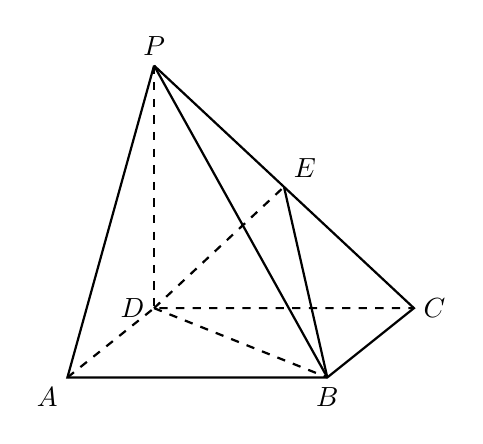
\begin{tikzpicture}[>=stealth, scale=1.1]
  % 顶点坐标
  \coordinate (D) at (1.0, 0.8);
  \coordinate (A) at (0, 0);
  \coordinate (B) at (3.0, 0);
  \coordinate (C) at (4.0, 0.8);
  \coordinate (P) at (1.0, 3.6);

  % 中点 E (PC 中点): P(1.0, 3.6), C(4.0, 0.8) -> E(2.5, 2.2)
  \coordinate (E) at (2.5, 2.2);

  % 实线棱
  \draw[thick] (P) -- (A) -- (B) -- (C) -- (P);
  \draw[thick] (P) -- (B);
  \draw[thick] (E) -- (B);

  % 虚线棱与辅助线
  \draw[dashed, thick] (P) -- (D);
  \draw[dashed, thick] (A) -- (D) -- (C);
  \draw[dashed, thick] (D) -- (B);
  \draw[dashed, thick] (D) -- (E);

  % 节点标注
  \node[above] at (P) {$P$};
  \node[below left] at (A) {$A$};
  \node[below] at (B) {$B$};
  \node[right] at (C) {$C$};
  \node[left] at (D) {$D$};
  \node[above right] at (E) {$E$};
\end{tikzpicture}
\end{center}
\nopagebreak[4]
（1）连接 $AC$ 与 $BD$ 相交于点 $O$。
因为底面 $ABCD$ 是正方形，所以对角线互相平分，点 $O$ 是 $AC$ 的中点。
连接 $EO$。
在 $\triangle PAC$ 中，$O$ 是 $AC$ 的中点，$E$ 是 $PC$ 的中点，
\Needspace{5\baselineskip}
所以 $EO$ 是 $\triangle PAC$ 的中位线，从而有：
\nopagebreak[4]
\[
PA \parallel EO.
\]
因为 $EO \subset \text{\text{平面} } EDB$，且 $PA \not\subset \text{\text{平面} } EDB$，
\Needspace{5\baselineskip}
由直线与平面平行的判定定理得：
\nopagebreak[4]
\[
PA \parallel \text{\text{平面} } EDB.
\]

（2）设正方形边长为 $a$，则 $PD = DC = a$。
取 $CD$ 的中点 $H$，连接 $EH$ 和 $BH$。
在 $\triangle PCD$ 中，$E$ 是 $PC$ 的中点，$H$ 是 $CD$ 的中点，
所以 $EH \parallel PD$，且 $EH = \dfrac{1}{2}PD = \dfrac{1}{2}a$。
\Needspace{5\baselineskip}
因为 $PD \perp \text{\text{底面} } ABCD$，所以：
\nopagebreak[4]
\[
EH \perp \text{\text{底面} } ABCD.
\]
从而 $HB$ 是斜线 $EB$ 在底面 $ABCD$ 上的射影，
$\angle EBH$ 即为直线 $EB$ 与底面 $ABCD$ 所成的角。
在底面正方形 $ABCD$ 中，$H$ 是 $CD$ 的中点，$\angle C = 90^\circ$，$BC = a, CH = \dfrac{1}{2}a$。
\Needspace{5\baselineskip}
在直角三角形 $\triangle BCH$ 中，由勾股定理：
\nopagebreak[4]
\[
BH = \sqrt{BC^2 + CH^2} = \sqrt{a^2 + \left(\dfrac{a}{2}\right)^2} = \dfrac{\sqrt{5}}{2}a.
\]
\Needspace{5\baselineskip}
在直角三角形 $\triangle EHB$ 中，$\angle EHB = 90^\circ$：
\nopagebreak[4]
\[
\tan\angle EBH = \dfrac{EH}{BH} = \dfrac{\dfrac{1}{2}a}{\dfrac{\sqrt{5}}{2}a} = \dfrac{1}{\sqrt{5}} = \dfrac{\sqrt{5}}{5}.
\]
即直线 $EB$ 与底面 $ABCD$ 所成角的正切值为 $\dfrac{\sqrt{5}}{5}$。

\gkanswer{答案：（1）证明见解析；（2）$\dfrac{\sqrt{5}}{5}$}

\end{answer}
\begin{answer}
\gksolhead{20}{}

\textbf{题目}（本小题满分 12 分）：

设 $\{a_n\}$ 是一个公差为 $d$ ($d \ne 0$) 的等差数列，它的前 10 项和 $S_{10} = 110$，且 $a_1, a_2, a_4$ 成等比数列．
（1）证明：$a_1 = d$；
（2）求公差 $d$ 的值和数列 $\{a_n\}$ 的通项公式．

\Needspace{4\baselineskip}
\textbf{解析}

（1）设等差数列 $\{a_n\}$ 的公差为 $d$ ($d \neq 0$)。
由等差数列通项性质，有 $a_2 = a_1 + d$，$a_4 = a_1 + 3d$。
\Needspace{5\baselineskip}
因为 $a_1, a_2, a_4$ 成等比数列，所以：
\nopagebreak[4]
\[
a_2^2 = a_1 a_4.
\]
\Needspace{5\baselineskip}
将通项代入上式：
\nopagebreak[4]
\[
(a_1 + d)^2 = a_1(a_1 + 3d) \iff a_1^2 + 2a_1 d + d^2 = a_1^2 + 3a_1 d.
\]
\Needspace{5\baselineskip}
整理得：
\nopagebreak[4]
\[
d^2 = a_1 d.
\]
\Needspace{5\baselineskip}
因为公差 $d \neq 0$，两边同除以 $d$，即证得：
\nopagebreak[4]
\[
a_1 = d.
\]

\Needspace{5\baselineskip}
（2）根据等差数列前 $n$ 项和公式：
\nopagebreak[4]
\[
S_{10} = 10a_1 + \dfrac{10 \times 9}{2}d = 10a_1 + 45d.
\]
\Needspace{5\baselineskip}
将 $a_1 = d$ 代入前 10 项和公式：
\nopagebreak[4]
\[
S_{10} = 10d + 45d = 55d.
\]
\Needspace{5\baselineskip}
已知 $S_{10} = 110$，故：
\nopagebreak[4]
\[
55d = 110 \implies d = 2.
\]
因此首项 $a_1 = d = 2$。
\Needspace{5\baselineskip}
数列 $\{a_n\}$ 的通项公式为：
\nopagebreak[4]
\[
a_n = a_1 + (n - 1)d = 2 + 2(n - 1) = 2n \quad (n \in \mathbf{N}^*).
\]

\gkanswer{答案：（1）证明见解析；（2）$d = 2$，$a_n = 2n$}

\end{answer}
\begin{answer}
\gksolhead{21}{}

\textbf{题目}（本小题满分 12 分）：

已知函数 $f(x) = ax^3 + cx + d$ ($a \ne 0$) 是 $\mathbf{R}$ 上的奇函数，当 $x = 1$ 时 $f(x)$ 取得极值 $-2$．
（1）求 $f(x)$ 的单调区间和极大值；
（2）证明：对任意 $x_1, x_2 \in (-1, 1)$，不等式 $|f(x_1) - f(x_2)| < 4$ 恒成立．

\Needspace{4\baselineskip}
\textbf{解析}

（1）已知函数 $f(x) = ax^3 + cx + d$ ($a \neq 0$) 是 $\mathbf{R}$ 上的奇函数。
由奇函数性质 $f(-x) = -f(x)$，得 $f(0) = 0$，即 $d = 0$。
故函数解析式为 $f(x) = ax^3 + cx$。
\Needspace{5\baselineskip}
求导数得：
\nopagebreak[4]
\[
f'(x) = 3ax^2 + c.
\]
\Needspace{5\baselineskip}
因为当 $x = 1$ 时 $f(x)$ 取得极值 $-2$，所以：
\nopagebreak[4]
\[
\begin{cases}
f'(1) = 3a + c = 0, \\
f(1) = a + c = -2.
\end{cases}
\]
\Needspace{5\baselineskip}
解得：
\nopagebreak[4]
\[
\begin{cases}
a = 1, \\
c = -3.
\end{cases}
\]
所以函数的解析式为 $f(x) = x^3 - 3x$。
\Needspace{5\baselineskip}
其导函数为：
\nopagebreak[4]
\[
f'(x) = 3x^2 - 3 = 3(x+1)(x-1).
\]
令 $f'(x) = 0$，解得驻点 $x_1 = -1, x_2 = 1$。
讨论单调性：
\begin{itemize}
\item 当 $x \in (-\infty, -1)$ 时，$f'(x) > 0$，$f(x)$ 单调递增；
\item 当 $x \in (-1, 1)$ 时，$f'(x) < 0$，$f(x)$ 单调递减；
\item 当 $x \in (1, +\infty)$ 时，$f'(x) > 0$，$f(x)$ 单调递增。
\end{itemize}
因此 $f(x)$ 的单调递增区间为 $(-\infty, -1)$ 和 $(1, +\infty)$；单调递减区间为 $(-1, 1)$。
\Needspace{5\baselineskip}
当 $x = -1$ 时取得极大值：
\nopagebreak[4]
\[
f(-1) = (-1)^3 - 3(-1) = -1 + 3 = 2.
\]

（2）由（1）可知，$f(x)$ 在开区间 $(-1, 1)$ 上连续且严格单调递减。
\Needspace{5\baselineskip}
所以对于任意 $x \in (-1, 1)$，其函数值满足：
\nopagebreak[4]
\[
f(1) < f(x) < f(-1) \iff -2 < f(x) < 2.
\]
\Needspace{5\baselineskip}
因此对任意 $x_1, x_2 \in (-1, 1)$，均有：
\nopagebreak[4]
\[
-2 < f(x_1) < 2, \quad \text{\text{且}} \quad -2 < f(x_2) < 2.
\]
\Needspace{5\baselineskip}
由不等式性质可得：
\nopagebreak[4]
\[
-2 < -f(x_2) < 2.
\]
\Needspace{5\baselineskip}
两式相加：
\nopagebreak[4]
\[
-4 < f(x_1) - f(x_2) < 4.
\]
\Needspace{5\baselineskip}
即：
\nopagebreak[4]
\[
|f(x_1) - f(x_2)| < 4.
\]
命题得证。

\gkanswer{答案：（1）单调递增区间为 $(-\infty, -1)$ 和 $(1, +\infty)$，单调递减区间为 $(-1, 1)$；极大值为 $2$；（2）证明见解析}

\end{answer}
\begin{answer}
\gksolhead{22}{}

\textbf{题目}（本小题满分 14 分）：

椭圆的中心是原点 $O$，它的短轴长为 $2\sqrt{2}$，相应于焦点 $F(c, 0)$ ($c > 0$) 的准线 $l$ 与 $x$ 轴相交于点 $A$，$|OF| = 2|FA|$，过点 $A$ 的直线与椭圆相交于 $P$、$Q$ 两点．
（1）求椭圆的方程及离心率；
（2）若 $\vec{OP} \cdot \vec{OQ} = 0$，求直线 $PQ$ 的方程．

\Needspace{4\baselineskip}
\textbf{解析}

（1）设椭圆的标准方程为 $\dfrac{x^2}{a^2} + \dfrac{y^2}{b^2} = 1$ ($a > b > 0$)。
由已知，短轴长为 $2\sqrt{2}$，即 $2b = 2\sqrt{2} \implies b = \sqrt{2} \implies b^2 = 2$。
焦点为 $F(c, 0)$ ($c > 0$)，相应准线 $l$ 的方程为 $x = \dfrac{a^2}{c}$。
因此准线与 $x$ 轴的交点坐标为 $A\left(\dfrac{a^2}{c}, 0\right)$。
\Needspace{5\baselineskip}
各线段长度为：
\nopagebreak[4]
\[
|OF| = c, \quad |FA| = \dfrac{a^2}{c} - c.
\]
\Needspace{5\baselineskip}
由已知条件 $|OF| = 2|FA|$ 得：
\nopagebreak[4]
\[
c = 2\left(\dfrac{a^2}{c} - c\right) \iff c^2 = 2a^2 - 2c^2 \iff 3c^2 = 2a^2 \iff \dfrac{c^2}{a^2} = \dfrac{2}{3}.
\]
\Needspace{5\baselineskip}
因此离心率为：
\nopagebreak[4]
\[
e = \dfrac{c}{a} = \sqrt{\dfrac{2}{3}} = \dfrac{\sqrt{6}}{3}.
\]
\Needspace{5\baselineskip}
由椭圆基本关系 $a^2 = b^2 + c^2 = 2 + \dfrac{2}{3}a^2$：
\nopagebreak[4]
\[
\dfrac{1}{3}a^2 = 2 \implies a^2 = 6.
\]
\Needspace{5\baselineskip}
所以椭圆的标准方程为：
\nopagebreak[4]
\[
\dfrac{x^2}{6} + \dfrac{y^2}{2} = 1.
\]

（2）由（1）知 $a^2 = 6, c^2 = 4 \implies c = 2$。
点 $A$ 的横坐标为 $x_A = \dfrac{a^2}{c} = \dfrac{6}{2} = 3$，即点 $A(3, 0)$。
若直线 $PQ \perp x$ 轴，则直线方程为 $x = 3$。但 $x_A = 3 > \sqrt{6} = a$，直线与椭圆没有公共点，
\Needspace{5\baselineskip}
因此直线 $PQ$ 的斜率存在，可设直线 $PQ$ 的方程为：
\nopagebreak[4]
\[
y = k(x - 3).
\]
\Needspace{5\baselineskip}
将直线方程代入椭圆方程 $\dfrac{x^2}{6} + \dfrac{y^2}{2} = 1 \iff x^2 + 3y^2 = 6$：
\nopagebreak[4]
\[
x^2 + 3k^2(x - 3)^2 = 6 \iff (1 + 3k^2)x^2 - 18k^2 x + 27k^2 - 6 = 0.
\]
设交点 $P(x_1, y_1), Q(x_2, y_2)$。
\Needspace{5\baselineskip}
直线与椭圆相交于不同两点，判别式必须大于 0：
\nopagebreak[4]
\[
\Delta = (-18k^2)^2 - 4(1 + 3k^2)(27k^2 - 6) = 324k^4 - 4(81k^4 + 9k^2 - 6) = 24 - 36k^2 > 0 \iff k^2 < \dfrac{2}{3}.
\]
\Needspace{5\baselineskip}
由一元二次方程根与系数的关系（韦达定理）：
\nopagebreak[4]
\[
x_1 + x_2 = \dfrac{18k^2}{1 + 3k^2}, \quad x_1 x_2 = \dfrac{27k^2 - 6}{1 + 3k^2}.
\]
\Needspace{5\baselineskip}
由于点 $P, Q$ 在直线上，纵坐标满足：
\nopagebreak[4]
\[
y_1 y_2 = k^2(x_1 - 3)(x_2 - 3) = k^2[x_1 x_2 - 3(x_1 + x_2) + 9].
\]
\Needspace{5\baselineskip}
将韦达定理结果代入括号内：
\nopagebreak[4]
\[
x_1 x_2 - 3(x_1 + x_2) + 9 = \dfrac{27k^2 - 6 - 54k^2 + 9(1 + 3k^2)}{1 + 3k^2} = \dfrac{3}{1 + 3k^2}.
\]
\Needspace{5\baselineskip}
因此：
\nopagebreak[4]
\[
y_1 y_2 = \dfrac{3k^2}{1 + 3k^2}.
\]
\Needspace{5\baselineskip}
由题设向量数量积 $\vec{OP} \cdot \vec{OQ} = 0$，等价于：
\nopagebreak[4]
\[
x_1 x_2 + y_1 y_2 = 0.
\]
\Needspace{5\baselineskip}
代入得：
\nopagebreak[4]
\[
\dfrac{27k^2 - 6}{1 + 3k^2} + \dfrac{3k^2}{1 + 3k^2} = 0 \iff 30k^2 - 6 = 0 \iff k^2 = \dfrac{1}{5}.
\]
经检验，$k^2 = \dfrac{1}{5} < \dfrac{2}{3}$，符合判别式条件。
\Needspace{5\baselineskip}
解得：
\nopagebreak[4]
\[
k = \pm \dfrac{\sqrt{5}}{5}.
\]
\Needspace{5\baselineskip}
所以直线 $PQ$ 的方程为：
\nopagebreak[4]
\[
y = \pm \dfrac{\sqrt{5}}{5}(x - 3) \iff x \pm \sqrt{5}y - 3 = 0.
\]

\gkanswer{答案：（1）$\dfrac{x^2}{6} + \dfrac{y^2}{2} = 1$，$e = \dfrac{\sqrt{6}}{3}$；（2）$y = \pm \dfrac{\sqrt{5}}{5}(x - 3)$（或 $x \pm \sqrt{5}y - 3 = 0$）}

\end{answer}